\chapter{Approach}

This chapter focuses on describing which approaches were chosen for the task at hand and why. 

To reiterate the current problem is to find out if \gls{gnn} can compete at solving the \gls{mwm} problem compared to other options such as greedy algorithm.

Before properly describing the choices made for approaching this problem, it is worth going through basic concepts of \gls{gnn}s and neural networks in general. It is common to think of neural networks as of a black box where you give some data to this box and it gives back an answer. In this case the data is a graph consisting of vertices connected by edges that have weights and the expected answer should be pairs of vertices that were matched together. This is however not as straight forward as the more common examples of classification where each data item needs to be classified.  

\section{Line graph approach}

Line graph approach was the first attempt at using a simple \gls{gnn}, which later turned out to be too time consuming for larger graphs to be worth further expriements. It did however give some usefull insight as well as a showed to be a proof of concept. In the context of graphs line graph is a complement of the original graph that turns each edge to a vertex and connects the vertices is they shared a vertex in the original graph. 

Examaple of a graph and its line graph convertion
\begin{figure}[H]
    \centering
    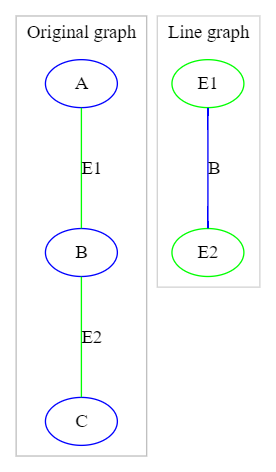
\includegraphics[scale=0.5]{figures/LineGraphExample}
    \caption{Original graph (left) and its line graph (right)}
  	\medskip 
	\hspace*{15pt}\hbox{\scriptsize Credit: my paint skills}
    \label{Line graph figure}
\end{figure}

\section{Edge classification approach}

The usual thing to do is for each pair of vertices that are conneced by an edge, ask the model if this pair should be a part of the matching. In other words model is classifying an edge. 

\section{Result Validation}

How good a solving method for \gls{mwm} is can be evaluated by:

\begin{enumerate}
\item Time - how long an algorithm took to produce an answer.
\item Correctness - is the answer correct. In case of \gls{mwm} the total weight aquired would be the measurement of how correct the solution is. It is unlikely that \gls{gnn} can find an optimal solution for more complex problems so it is reasonable to look at how close \gls{gnn} comes to the optimal solution.
\item Memory - how much memory is needed. However in this project there is less of a focus on memory
\end{enumerate}
